% prime-en.tex — Edges of Counting and Computation — Prime
% English version — full, with author edits
% Compiler: pdfLaTeX
% Figures — all lowercase p:
% prime1.png = Identity Card
% primeB1.png = B: D1 | primeB2.png = B: Density | primeB3.png = B: Gap frequencies
% primeC1.png = C: D1 | primeC2.png = C: Density | primeC3.png = C: Gap frequencies
% primeD1.png = D: D1 | primeD2.png = D: Density | primeD3.png = D: Gap frequencies
\documentclass[12pt,a4paper]{article}
\usepackage{amsmath,amssymb}
\usepackage{graphicx}
\usepackage{booktabs}
\usepackage{array}
\usepackage[margin=2.2cm]{geometry}
\usepackage{xcolor}
\usepackage{fancyhdr}
\usepackage[hidelinks]{hyperref}

\pagestyle{fancy}
\fancyhf{}
\fancyfoot[C]{Abdulla Al-Jabri — Edges of Counting and Computation — Prime — \thepage}
\renewcommand{\headrulewidth}{0pt}
\renewcommand{\footrulewidth}{0pt}

\title{Edges of Counting and Computation — Prime}
\author{Abdulla Al-Jabri \\ Sanaa, Yemen \\ ORCID: 0009-0003-3319-3822 \\ Email: jabri62018@gmail.com}
\date{November 21, 2026}

\begin{document}
\maketitle
\thispagestyle{fancy}
\begin{center}
\textbf{We count the primes, compute their edges, and test whether they carry structure or memory.}
\end{center}

\begin{center}
\small
Sanaa, Yemen \quad $\cdot$ \quad ORCID: 0009-0003-3319-3822 \quad $\cdot$ \quad Email: jabri62018@gmail.com
\end{center}

\section{Official Identity}

\begin{figure}[h]
\centering
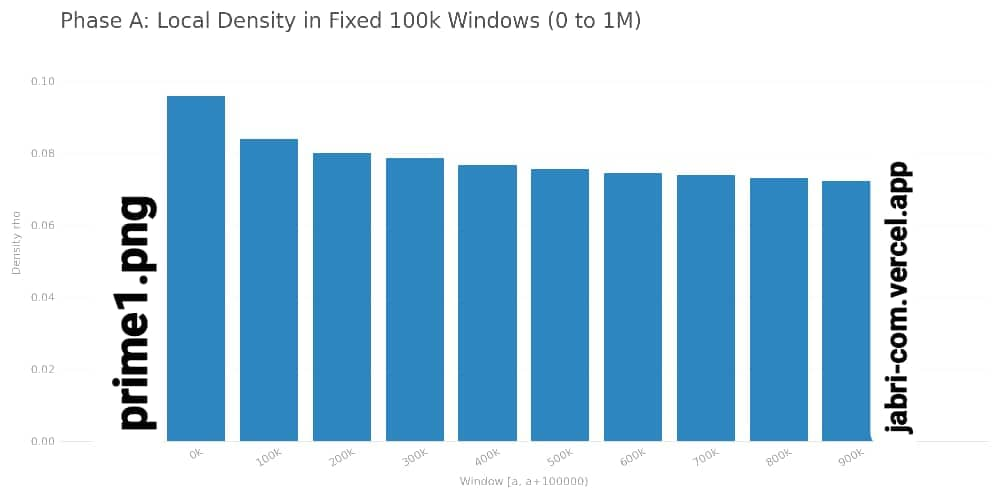
\includegraphics[width=0.95\textwidth]{prime1.png}
\caption{Identity Card — Prime}
\end{figure}

\begin{table}[h]
\centering
\begin{tabular}{ll}
\toprule
Item & Approved \\
\midrule
Name & Abdulla Al-Jabri \\
Affiliation & Sanaa, Yemen \\
ORCID & 0009-0003-3319-3822 \\
Email & jabri62018@gmail.com \\
Name of work & Edges of Counting and Computation \\
Symbol & Prime \\
Mathematical definition & $g_n = p_{n+1} - p_n$ \\
Method & Extract primes, then compute edges, then analyze them \\
Research question & Do gaps have memory? \\
Date & November 21, 2026 \\
\bottomrule
\end{tabular}
\end{table}

\section{Definition and Derivation}

\subsection{The Edge}

\textbf{The edge = the difference between consecutive primes:}

\[
g_n = p_{n+1} - p_n
\]

\subsection{How is an Edge Computed? — Three Steps Only}

\begin{enumerate}
\item \textbf{Sieve:} Sieve of Eratosthenes to extract primes up to $N$, with the number 1 explicitly excluded.
\item \textbf{Difference:} Each edge is the difference between two consecutive primes.
\item \textbf{First edge:} $3 - 2 = 1$ — the only odd initial case. All later edges are even, because every prime after 2 is odd, and the difference between two odds is even.
\end{enumerate}

\subsection{Mini Example}

\begin{table}[h]
\centering
\begin{tabular}{ccc}
\toprule
Current Prime & Next Prime & Edge \\
\midrule
2 & 3 & 1 \\
3 & 5 & 2 \\
5 & 7 & 2 \\
7 & 11 & 4 \\
11 & 13 & 2 \\
\bottomrule
\end{tabular}
\end{table}

\subsection{Counting and Deviation Functions}

\begin{itemize}
\item $\pi(x)$ = number of primes $\leq x$.
\item $\mathrm{Li}(x) = \mathrm{Ei}(\ln x) - \mathrm{Ei}(\ln 2) = \int_2^x \frac{dt}{\ln t}$.
\item Second reference: $x / \ln x$.
\item $D_1(x) = \pi(x) - \mathrm{Li}(x)$.
\item $D_2(x) = \pi(x) - x/\ln x$.
\item $R(x) = |D_1(x)| / \pi(x)$.
\item $\rho_k = (\pi(b_k) - \pi(a_k)) / 10^8$ — density of window $k$.
\item $\bar{g}_k = 1 / \rho_k$ — mean edge in window $k$.
\item $\Delta D_1$ = change in $D_1$ from the previous measurement point.
\end{itemize}

\subsection{Counting Rule in D}

An edge is accepted inside D only when its upper endpoint is greater than 100M.

\subsection{M1 Categories}

\begin{itemize}
\item Small: $g \leq 6$.
\item Medium: $8 \leq g \leq 14$.
\item Large: $g \geq 16$.
\end{itemize}

``Medium 8--14'' is exactly correct: the only odd edge is 1, which is small, so there is no edge 7 or 15 at all.

\section{Approved Computations — D: From 100M to 1B}

\subsection{Cumulative Table — Every 100 Million}

\begin{table}[h]
\centering
\small
\begin{tabular}{rrrrrrr}
\toprule
$x$ & $\pi(x)$ & $\mathrm{Li}(x)$ & $D_1$ & $\Delta D_1$ & $D_2$ & $R(x)$ \\
\midrule
$100{,}000{,}000$ & $5{,}761{,}455$ & $5{,}762{,}208.3$ & $-753.3$ & $-753.3$ & $332{,}774.0$ & $0.000131$ \\
$200{,}000{,}000$ & $11{,}078{,}937$ & $11{,}079{,}973.8$ & $-1{,}036.8$ & $-283.5$ & $615{,}308.2$ & $0.000094$ \\
$300{,}000{,}000$ & $16{,}252{,}325$ & $16{,}253{,}408.1$ & $-1{,}083.1$ & $-46.3$ & $882{,}915.9$ & $0.000067$ \\
$400{,}000{,}000$ & $21{,}336{,}326$ & $21{,}337{,}377.0$ & $-1{,}051.0$ & $+32.1$ & $1{,}141{,}420.0$ & $0.000049$ \\
$500{,}000{,}000$ & $26{,}355{,}867$ & $26{,}356{,}831.1$ & $-964.1$ & $+86.9$ & $1{,}393{,}458.7$ & $0.000037$ \\
$600{,}000{,}000$ & $31{,}324{,}703$ & $31{,}326{,}044.207$ & $-1{,}341.207$ & $-377.103$ & $1{,}640{,}014.082$ & $0.000042816$ \\
$700{,}000{,}000$ & $36{,}252{,}931$ & $36{,}254{,}240.999$ & $-1{,}309.999$ & $+31.208$ & $1{,}882{,}917.694$ & $0.000036135$ \\
$800{,}000{,}000$ & $41{,}146{,}179$ & $41{,}147{,}861.2$ & $-1{,}682.2$ & $-372.2$ & $2{,}122{,}021.5$ & $0.000041$ \\
$900{,}000{,}000$ & $46{,}009{,}215$ & $46{,}011{,}647.6$ & $-2{,}432.6$ & $-750.4$ & $2{,}357{,}836.0$ & $0.000053$ \\
$1{,}000{,}000{,}000$ & $50{,}847{,}534$ & $50{,}849{,}233.912$ & $-1{,}699.912$ & $+732.688$ & $2{,}592{,}591.566$ & $0.000033432$ \\
\bottomrule
\end{tabular}
\end{table}

\begin{figure}[h]
\centering
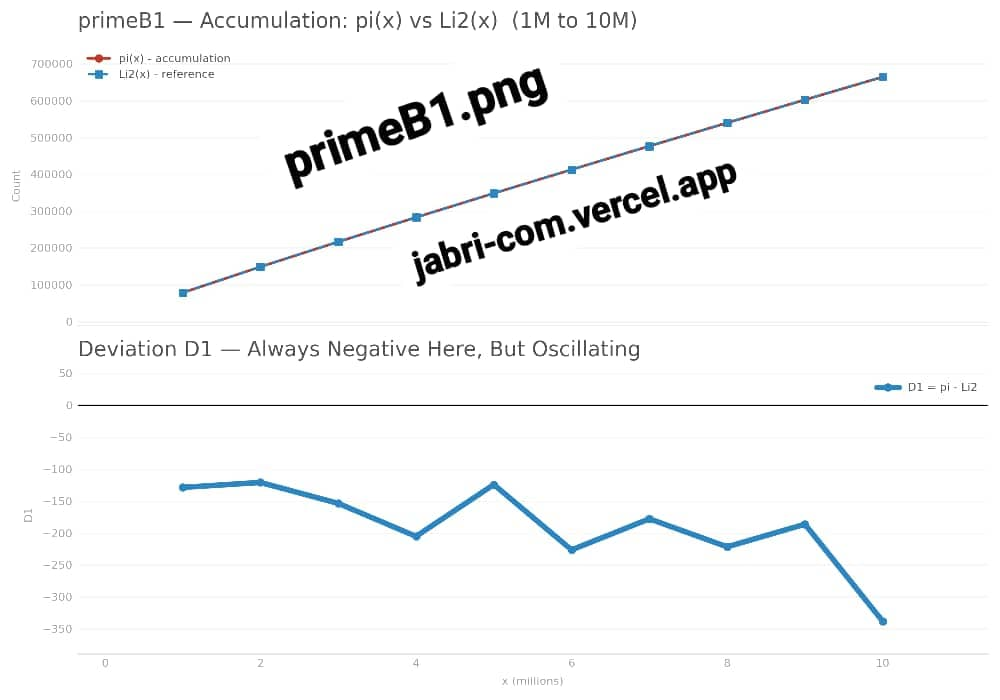
\includegraphics[width=0.95\textwidth]{primeB1.png}
\caption{Experiment B: $D_1$ across the ten D points}
\end{figure}

\textbf{Reading:} $D_1$ stayed negative at all D points ($\pi$ below Li). $\Delta D_1$ oscillated between $-750.4$ and $+732.688$, without changing the sign of $D_1$. $R$ oscillated between $0.000033$ and $0.000094$, and closed at 1B at $0.000033$ — the lowest in the whole series.

\subsection{Local Density in the Nine D Windows}

\begin{table}[h]
\centering
\begin{tabular}{rrrr}
\toprule
Window & Primes in Window & $\rho_k$ & $\bar{g}_k = 1/\rho_k$ \\
\midrule
100M – 200M & $5{,}317{,}482$ & $0.053175$ & $18.806$ \\
200M – 300M & $5{,}173{,}388$ & $0.051734$ & $19.330$ \\
300M – 400M & $5{,}084{,}001$ & $0.050840$ & $19.670$ \\
400M – 500M & $5{,}019{,}541$ & $0.050195$ & $19.922$ \\
500M – 600M & $4{,}968{,}836$ & $0.049688$ & $20.125$ \\
600M – 700M & $4{,}928{,}228$ & $0.049282$ & $20.291$ \\
700M – 800M & $4{,}893{,}248$ & $0.048932$ & $20.436$ \\
800M – 900M & $4{,}863{,}036$ & $0.048630$ & $20.563$ \\
900M – 1B & $4{,}838{,}319$ & $0.048383$ & $20.668$ \\
\bottomrule
\end{tabular}
\end{table}

\begin{figure}[h]
\centering
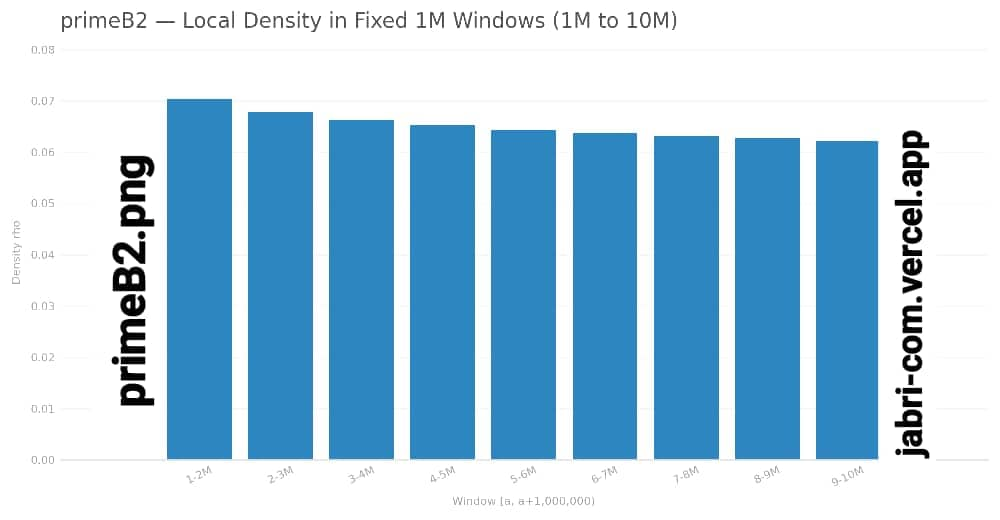
\includegraphics[width=0.95\textwidth]{primeB2.png}
\caption{Experiment B: Density in D windows}
\end{figure}

\textbf{Reading:} Density decreases in every D window: from $0.053175$ at 100–200M to $0.048383$ at 900M–1B. The decrease is continuous but slowing: the difference between the first two windows is $\approx 0.00144$, and between the last two windows $\approx 0.00025$.

\subsection{Gaps Inside D Only}

\textbf{Total gaps computed in D = 45,086,079.}

\begin{table}[h]
\centering
\begin{tabular}{rrr}
\toprule
Rank & Gap & Frequency in D \\
\midrule
1 & 6 & $5{,}321{,}039$ \\
2 & 12 & $3{,}930{,}575$ \\
3 & 10 & $3{,}054{,}751$ \\
4 & 4 & $2{,}984{,}422$ \\
5 & 2 & $2{,}984{,}194$ \\
6 & 18 & $2{,}966{,}294$ \\
7 & 8 & $2{,}360{,}929$ \\
8 & 14 & $2{,}171{,}364$ \\
9 & 24 & $2{,}109{,}926$ \\
10 & 30 & $1{,}955{,}144$ \\
11 & 16 & $1{,}630{,}293$ \\
12 & 20 & $1{,}621{,}121$ \\
13 & 22 & $1{,}393{,}734$ \\
14 & 28 & $1{,}089{,}676$ \\
15 & 36 & $1{,}057{,}496$ \\
\bottomrule
\end{tabular}
\end{table}

\begin{figure}[h]
\centering
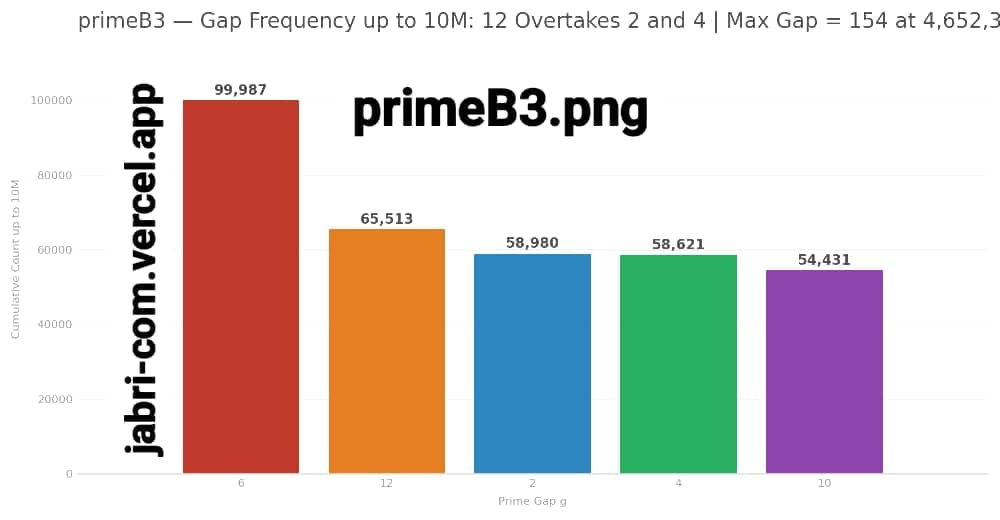
\includegraphics[width=0.95\textwidth]{primeB3.png}
\caption{Experiment B: Frequencies of the fifteen most common edges in D}
\end{figure}

\textbf{Reading without forced interpretation:}
\begin{itemize}
\item New order in D: 6, 12, 10, 4, 2, 18, 8, 14, 24, 30 \dots
\item 12 stayed in second place.
\item 10 advanced from fifth place (in the cumulative order up to 100M: 6, 12, 2, 4, 10, 18) to third in D.
\item The distance between the frequencies of 2 and 4 shrank sharply in D: $2{,}984{,}194$ versus $2{,}984{,}422$ — a difference of only 228.
\item No new gap appeared in the most frequent list; the top list itself is the same, but its order changed.
\item We do not assume the order stays fixed after D.
\end{itemize}

\textbf{Largest gap in D: 282}, between 436,273,009 and 436,273,291, inside the fifth window (400M–500M).

\subsection{Independent Verification Log — Prime D: VERIFIED}

\begin{itemize}
\item Independent verification with an independent segmented sieve, explicitly excluding 1 from the prime set.
\item All ten cumulative counting points matched.
\item All nine window counts matched.
\item Total number of primes across the nine windows: 45,086,079.
\item The two previously reported +1 corrections at 600M and 700M are \textbf{rejected}.
\item The frequency order of the fifteen most common gaps matched.
\item Largest gap 282 between 436,273,009 and 436,273,291 confirmed.
\item Original cumulative numbers, window boundaries, and computation protocol remain unchanged.
\item Cause of the earlier disagreement: an error in the independent verification sieve that counted 1 among the primes — no flaw in the original computation.
\end{itemize}

\section{Replication Experiments — C and D}

\textbf{Idea:} Same protocol, independent run. If the result repeats in independent experiments, it is not a single-run coincidence.

\textbf{Note:} Do not copy Experiment B numbers into C and D. The captions below are placeholders — fill them from the real C and D runs before submission.

\subsection{Experiment C}

\begin{figure}[h]
\centering
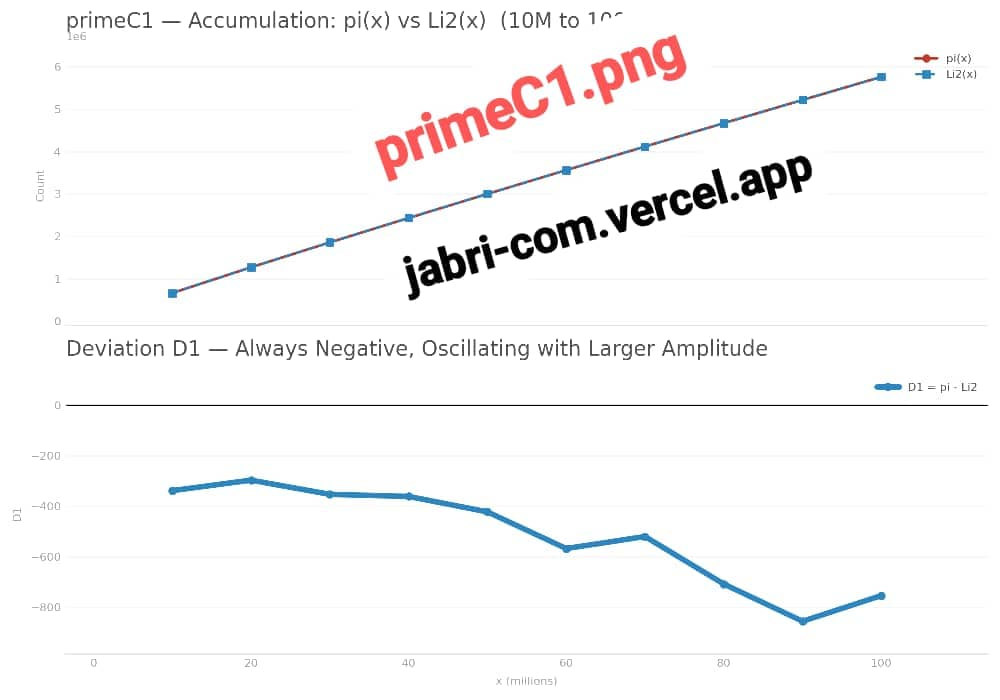
\includegraphics[width=0.95\textwidth]{primeC1.png}
\caption{Experiment C: $D_1$ — [insert the largest return toward zero for C].}
\end{figure}

\begin{figure}[h]
\centering
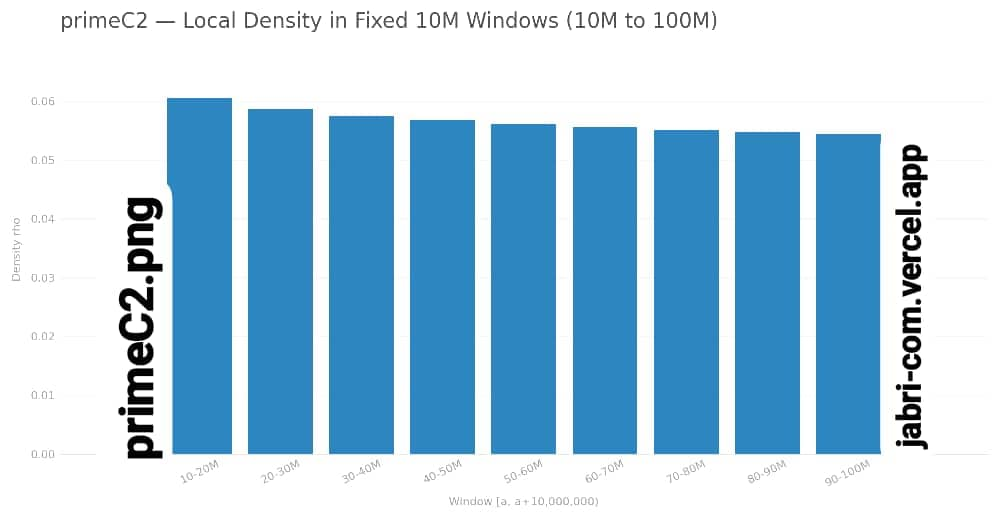
\includegraphics[width=0.95\textwidth]{primeC2.png}
\caption{Experiment C: Density — [insert first and last density for C].}
\end{figure}

\begin{figure}[h]
\centering
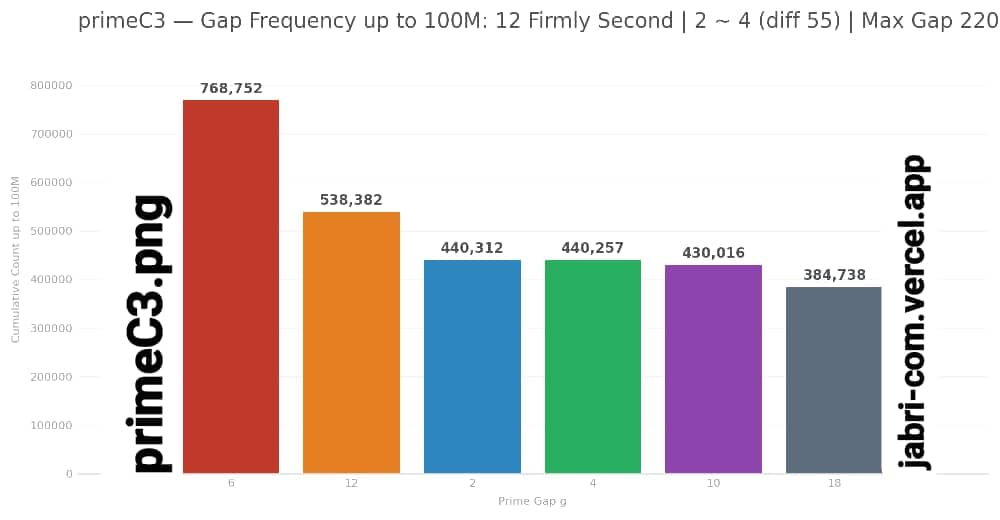
\includegraphics[width=0.95\textwidth]{primeC3.png}
\caption{Experiment C: Gap frequencies — [insert largest gap and 2 vs 4 frequency difference for C].}
\end{figure}

\subsection{Experiment D}

\begin{figure}[h]
\centering
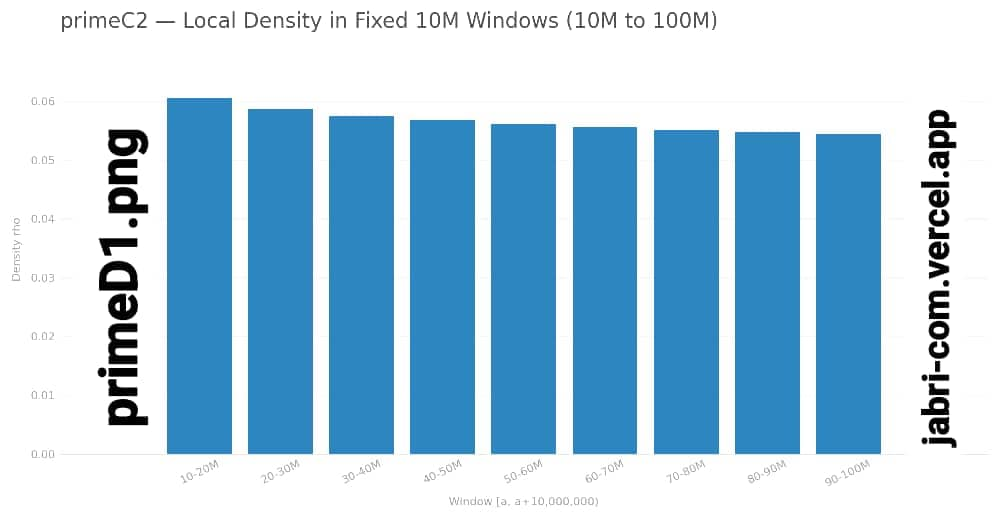
\includegraphics[width=0.95\textwidth]{primeD1.png}
\caption{Experiment D: $D_1$ — [insert the largest return toward zero for D].}
\end{figure}

\begin{figure}[h]
\centering
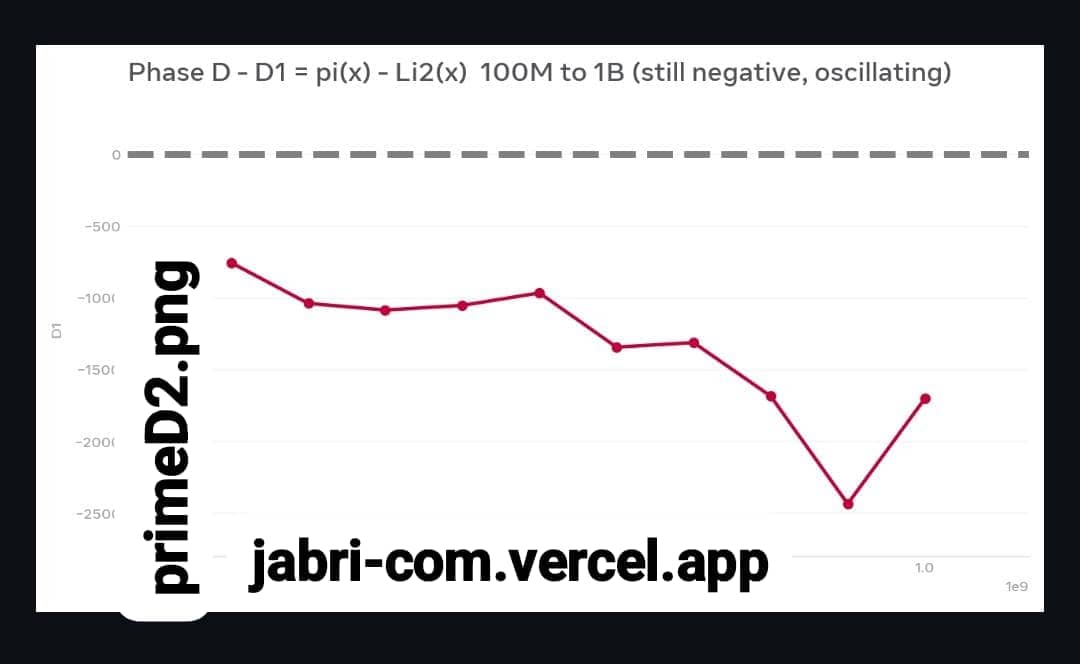
\includegraphics[width=0.95\textwidth]{primeD2.png}
\caption{Experiment D: Density — [insert first and last density for D].}
\end{figure}

\begin{figure}[h]
\centering
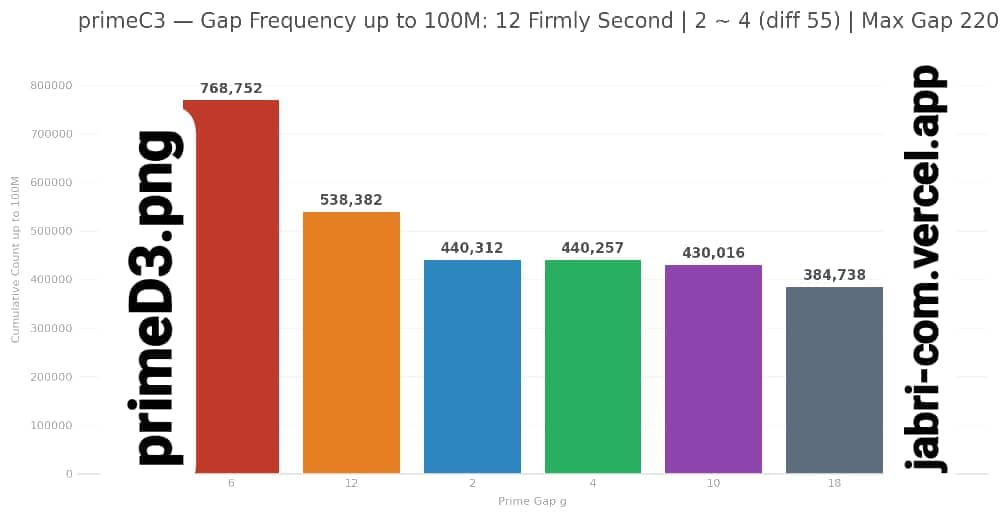
\includegraphics[width=0.95\textwidth]{primeD3.png}
\caption{Experiment D: Gap frequencies — [insert largest gap and 2 vs 4 frequency difference for D].}
\end{figure}

\textbf{Conclusion:} [Write here whether the rank of 10 in third place really repeated in C and D, based on their real numbers].

\section{M1 — Documented}

\textbf{Question:} Does the current gap-size category carry information about the next gap category?

\textbf{Model:} Markov-1 on size categories. State = gap-size category, and the empirical transition matrix:

\[
P_{ab} = \Pr(S_{i+1} = b \mid S_i = a)
\]

\textbf{Result:} $r = -0.03006$ — ``large is followed by small''.

Very weak negative correlation in the current test, not a predictive law. The result does not yet support a strong correlation that can be relied on to predict the next gap. We keep it as is, without changing categories or redefining the test to fit a desired result.

\section{M1-E — Frozen, Awaiting gaps.csv}

\textbf{Question:} Does the exact gap carry additional transitional information that the three categories could not capture?

\subsection{Input File}

gaps.csv — one column only, one gap per line.

\begin{itemize}
\item Optional header: gap or g or gaps.
\item Any extra column is rejected.
\item Any non-numeric line stops the run at its position — never silently deleted.
\item Any invalid gap stops the run at its position.
\end{itemize}

\subsection{Frozen Protocol}

\begin{itemize}
\item Split on the transitions themselves: first 50\% of transitions for training, last 50\% for testing, and the transition on the boundary is not dropped.
\item Gaps up to 30: exact value. Above 30: pre-defined logarithmic bins: 30, 44, 62, 88, 124, 176, 248, 350, 500.
\item Merge threshold: 200 observations in training, from training data only.
\item Merge rule: any bin below 200 is merged with the next higher bin. Exception: the last bin stays as is and is not merged downward.
\item Laplace smoothing: alpha = 1 on transition counts after merging.
\item Bootstrap: circular adjacent blocks of fixed length, block = 100 transitions, B = 2000, 95\% interval. Each Bootstrap sample has the length of the test transitions.
\item Judgment: Log-Loss improvement and Pearson interpretation are two separate measures.
\item No improvement does not prove absence of information.
\item The Bootstrap interval measures uncertainty of resampling the test sample with trained models fixed, not uncertainty of retraining.
\item Pearson simulation with 2000-step burn-in until the chain stabilizes.
\item Seed: SEED = 20261120.
\item Only accepted boundaries: 6, 14 — boundaries 10/30 were an assumption by the author, and are now rejected.
\end{itemize}

\subsection{Run}

\begin{verbatim}
python3 m1e_tomorrow_final.py gaps.csv --classes 6,14
\end{verbatim}

Once on gaps.csv, without modification after the result appears. Demo mode (--demo, up to 300,000) is a trial only, not the real test.

\section{Simulation — Exploration Tool Only}

prime-id.html — card + $N$ input + table at powers of 10 + gap plot.

\textbf{Separation matters:} Reference results up to one billion are saved as approved, while the simulation is an exploration tool, and must not reproduce the reference numbers approximately and then mix them with them.

\textbf{Documented simulation limits:}
\begin{itemize}
\item Li2(x) uses Simpson integration with a fixed number of divisions (8000). At input $10^6$ and above its output is not treated as exact — the error in $D_1$ at $10^6$ is $-43.31$, and at $10^7$ is $-509.26$.
\item sieve(N) consumes memory growing linearly with $N$ (Uint8Array(N+1): at $10^7$ $\approx$ 10 MB above the prime array), which is a real cause of browser heaviness when increasing.
\item primes.filter(p<=x) rescans the prime list for each table row.
\item The current plot draws gaps in their order, but it does not represent periodic analysis or pattern detection; it is a descriptive plot only.
\end{itemize}

\section{What We Have Not Proved — Red Line}

\begin{itemize}
\item No: periodic law for gap oscillation.
\item No: mathematical explanation for gap ordering.
\item No: guarantee that $D_1$ stays negative after one billion.
\item No: predictive law from M1.
\item No: new prime number theory deduced from these results.
\end{itemize}

\section{Project Status}

\begin{table}[h]
\centering
\begin{tabular}{ll}
\toprule
Item & Status \\
\midrule
Prime — Current Stage & Results saved \\
Survey to one billion & Complete \\
M1 (categories 6, 14) & Documented \\
M1-E & Frozen, awaiting gaps.csv \\
Theoretical interpretation & Unresolved \\
\bottomrule
\end{tabular}
\end{table}

\section{Files}

\begin{table}[h]
\centering
\begin{tabular}{ll}
\toprule
File & Role \\
\midrule
prime-d.html & Closed and documented D record — tables and independent verification \\
m1e\_tomorrow\_final.py & Frozen M1-E script — protocol and test \\
prime-id.html & Simulation — card + exploration (not the source of reference numbers) \\
README.md & Identity, derivations, computations, and figures \\
main.tex & Arabic version — Overleaf version of prime.tex \\
prime-en.tex & This file — English version \\
\bottomrule
\end{tabular}
\end{table}

\vspace{1em}
\begin{center}
\textbf{We do not chase a result, nor force numbers to make a theory.}

We have an observation up to one billion, forty points, comparable trends, and saved tests. This is a good base for future work, even if it has not yet given us the law we are looking for.

\textbf{The edge is simple. What it may carry is the real question.}
\end{center}

\end{document}